\chapter{Opis wymagań}
Istotą tego rozdziału jest opisanie wszystkich wymagań stawianych tworzonej bibliotece. 
Rozdział ten składa się z~dwóch głównych części: opisu wymagań funkcjonalnych i~opisu wymagań pozafunkcjonalnych.

Opis wymagań funkcjonalnych rozpoczynają wymagania stawiane całej bibliotece oraz wymagania odnoszące się do wszystkich tworzonych za jej pomocą wykresów. Następnie zostały przedstawione specyficzne wymagania dotyczące konkretnych typów wykresów.

Opis wymagań pozafunkcjonalnych został dokonany w~kontekście całej biblioteki, a~w~jego skład wchodzą rozważania na temat takich zagadnień jak skalowalność, wydajność czy niezawodność.

%\section{Wspólne wymagania funkcjonalne}

\section{Wykresy biurowe}
Za pomocą projektowanej biblioteki programiści będą mieć możliwość tworzenia interaktywnych wykresów typu biurowego. Po lekturze rozdziału poświęconego przeglądowi dziedziny wiadomo już, że zbiór wykresów biurowych jest dość liczny. Z~drugiej strony łatwo zauważyć, że jeden podzbiór wykresów jest szczególnie popularny. Projektując tę bibliotekę staram się skupić na stworzeniu elastycznej architektury, a~nie na udostępnieniu jak największej liczby typów wykresów. W~pierwszej wersji biblioteki zbiór wykresów będzie dośc ubogi i~będzie zawierał jedynie te najpopularniejsze.

\subsection{Dostępne wykresy}
Biblioteka musi udostępniać następujące typy wykresów:
\begin{itemize}
\item{kołowy,}
\item{słupkowy,}
\item{liniowy.}
\end{itemize}

%Specyficzne wymagania dotyczące wykresów każdego z~tych typów zostały podane w~dalszej części rozdziału.

\subsection{Inne wykresy}
Architektura biblioteki musi umożliwiać dodawanie nowych typów wykresów biurowych. Mechanizmy takie jak współpraca ze źródłami danych lub podłączenie widoku do wykresu powinny być na tyle uniwersalne, aby nie wymagały jakichkolwiek modyfikacji dla wykresów nowych typów. W~idealnym scenariuszu stworzenie nowego wykresu powinno ograniczyć się do zaimplementowania jego wewnętrznej logiki oraz wykorzystania już istniejących komponentów, np. legendy, bez ich modyfikacji.
 
\section{Uniwersalny silnik}
Podstawowym celem projektowanej biblioteki jest udostępnienie programistom uniwersalnego silnika umożliwiającego tworzenie interaktywnych wykresów. Ma to być rozwiązanie generyczne, działające zarówno dla klasycznego Qt jak i~Qt~Quick~2. Tworzony silnik powinien umożliwiać wyświetlenie wykresów w~następujących miejscach:
\begin{itemize}
\item{widgety,}
\item{architektura Graphics View,}
\item{dokumenty tekstowe,}
\item{QML.}
\end{itemize}

W~tablicy~\ref{tab:widoki} zostały podane stosowne dla każdego z~przypadków wykorzystania widoki.

\begin{table}[h]\footnotesize
\centering
\caption{Widoki kompatybilne z~moją biblioteką}
\label{tab:widoki}
\begin{tabular}{|c|c|}
\hline
Miejsce & Klasa bazowa widoku\\
\hline
Widget & QWidget\\
\hline
Graphics View & QGraphicsObject\\
\hline
Dokument tekstowy & QTextFrame\\
\hline
QML & QQuickItem -- klasy bazujące na SceneGraph\\
 & QQuickPaintedItem -- klasy bazujące na QPainter\\
\hline
\end{tabular}
\end{table}


\section{Źródła danych}
Typowym źródłem danych jest seria, czyli swego rodzaju pojemnik na próbki. Każde źródło danych, którym ma być zasilany wykres, musi udostępniać zbiór danych o~następującej strukturze:

\begin{itemize}
\item{jedna liczba ze specyficznego dla danego przypadku zbioru wartości, będącego podzbiorem zbioru liczb rzeczywistych,}
\item{co najmniej jedna wartość z~dziedziny liczb rzeczywistych. Bardziej złożone wykresy mogą mieć kilka takich wartości,}
\item{tytuł próbki,}
\item{kolor.}
\end{itemize}

Zakładam, że serie zawierają maksymalnie jedną próbkę dla danego wektora z~dziedziny. 

Ponadto wymagany jest tytuł i~kolor dla każdej z~serii.


\subsection{Serie danych}
Istnieje potrzeba stworzenia prostego i~lekkiego modelu danych reprezentującego serie, które z~kolei zawierają próbki. Niezbędne są operacje dodawania, modyfikowania i~usuwania danych z~serii. 

Aby ułatwić programistom Qt zapoznanie się ze sposobem działania mojej biblioteki, powinienem skorzystać tutaj ze statycznego polimorfizmu. Interfejs serii danych powinien przypominać interfejs modelu z~architektury Model-Widok.

\subsection{Model--Widok}
Wykresy mają być alternatywą dla widoków z~architektury Model-Widok. Uważam, że typowym przypadkiem użycia będzie prezentowanie tych samych danych za pomocą wykresów oraz tabelek. Z~tego powodu wszystkie wykresy muszą przyjmować jako źródło danych obiekty klas dziedziczących po \textit{QAbstractItemModel}.

%\subsection{Modele w QML}
%Szczególnymi przypadkami modeli są te wykorzystywane w~QML. Ważne jest, aby podłączenie elementów \textit{ListModel}~\footnote{ListModel \url{http://qt-project.org/doc/qt-5.1/qtqml/qml-qtqml-models2-listmodel.html}} i~\textit{XmlListModel}~\footnote{XmlListModel \url{http://qt-project.org/doc/qt-5.0/qtquick/qml-qtquick-xmllistmodel2-xmllistmodel.html}} do wykresu było intuicyjne dla programistów QML i~ograniczało się do jednej operacji:
%\begin{lstlisting}
%model: xmlModel
%\end{lstlisting}

\section{Interaktywność}
Celem tej pracy jest stworzenie biblioteki ,,do operowania na wykresach''. Wszystkie wykresy muszą obsługiwać interaktywne operacje, a~część z~nich powinna zostać zaimplementowana. Pozostałe powinny być możliwe do realizacji.

\subsection{Zaznaczanie}
Musi istnieć możliwość zaznaczania elementów reprezentujących dane. Powinna istnieć możliwość zaznaczania zarówno elementów reprezentujących pojedyncze próbki, np. wycinek kołowy, jak i~tych tych odpowiadających całym seriom danych, np. grupa słupków. Zaznaczanie powinno być możliwe poprzez kliknięcie przyciskiem myszy lub dotknięcie ekranu dotykowego.

\subsection{Modyfikacja zawartości modelu}
Powinna istnieć możliwość zmiany zawartości modelu poprzez interakcję z~wykresem. Dla danego elementu reprezentującego próbkę, zmiana jego parametru proporcjonalnego do reprezentowanej wartości powinna skutkować zmianą danych zawartych w~modelu. I~tak, skrócenie słupka powinno spowodować zmniejszenie odpowiedniej wartości w~modelu, a~zwiększenie kąta rozwarcia wycinka kołowego zwiększenie analogicznej wartości.

\subsection{Inne operacje}
Architektura biblioteki powinna umożliwiać programistom realizację innych interaktywnych operacji, np. system \textit{Przeciągnij i~Upuść}. Powinno być to możliwe poprzez wykorzystanie systemu zdarzeń Qt.

%\subsection{API w stylu Qt}


\section{Qt~Quick}
Projektując tę bibliotekę muszę wziąć pod uwagę jej późniejsze zastosowanie, którym ma być m.in. tworzenie wykresów w~QML. Projekt powinien zawierać również popularny w~QML mechanizm delegatów.

\subsection{Wyeksponowanie klas C++ w QML}
Już na etapie projektowania należy zadbać, aby tworzone struktury były łatwe do wyeksponowania w~QML. 
Tworzenie interfejsów do QML nie jest celem tego projektu, jednak ich implementacja powinna być możliwie łatwa dla programistów decydujących się na korzystanie z~mojej biblioteki.

\subsection{Delegaty}
Szeroko stosowanym w~Qt~Quick mechanizmem są delegaty. Umożliwiają one zdefiniowanie przez programistę sposobu prezentacji danych z~modelu. W~mojej bibliotece korzystanie z~delegatów powinno być możliwe w~legendzie, do prezentacji kolorów, oraz we właściwym wykresie do definiowania własnych elementów prezentujących zawartość modelu, np. słupki.


\section{Wspólne elementy składowe}
Wszystkie wykresy muszą zawierać następujące elementy:
\begin{itemize}
\item{źródło danych,}
\item{elementy prezentujące pojedyncze próbki danych (słupek, punkt, wycinek kołowy),}
\item{tytuł wykresu,}
\item{legenda,}
\item{dodatkowe elementy dostarczane przez programistów.}
\end{itemize}

Wyświetalnie każdego z~elementów wykresu powinno być sterowane przez programistę. Powinna również istnieć możliwość ustawienia tła wykresu.

 
\subsection{Elementy prezentujące dane}
Każdy z~wykresów posiada specyficzny dla niego element służący do prezentacji danych z~próbki, którego rozmiar lub położenie w~układzie współrzędnych odzwierciedla wartość próbki. Każdy z~elementów może mieć swój podpis. Powinna istnieć możliwość ustawienia tym elementom dwóch piór i~dwóch pędzli -- dla trybu normalnego i~zaznaczenia. Programista powinien mieć możliwość podmiany, dla danego wykresu, klasy takiego elementu na własną, przy czym odpowiedzialność za poprawne odrysowanie się wykresu spada wtedy na programistę.

\subsection{Tytuł wykresu i podpisy elementów}
Dla wszelkich napisów będących składowymi wykresu musi być możliwość ustawienia ich treści, czcionki oraz koloru.

\subsection{Legenda}
Dla wykresów obsługujących wiele serii danych legenda powinna prezentować kolory oraz tytuły tych serii. Natomiast dla wykresów jednoseryjnych prezentowana powinna być informacja o~kolorze i~tytule każdej z~próbek. Legenda powinna przyjmować jedno z~dwóch położeń -- poziome lub pionowe. Powinna istnieć możliwość zmiany elementu prezentującego kolor za pomocą mechanizmu delegatów.

\subsection{Dodatkowe elementy}
Programiści powinni mieć możliwość tworzenia własnych elementów i~dodawania ich do wykresów już istniejących klas. Aby to osiągnąć powinni jedynie zaimplementować odpowiednie interfejsy.


%\section{Dostępne operacje na wykresach}
\section{Skalowanie}
Powinno być możliwe skalowanie wykresu. Wykres powinien dostosowywać swój rozmiar do przekazanego mu obszaru przeznaczonego na jego odrysowanie.



\section{Wykresy w układzie współrzędnych}
Niektóre wykresy wymagają osadzenia w~układzie współrzędnych. Takie wykresy wymagają dodatkowych elementów:

\begin{itemize}
\item{osie,}
\item{siatka.}
\end{itemize}

\subsection{Osie}
Powinna istnieć możliwość przypisania do osi skali innej niż liniowa.
Powinna być możliwość ustawienia pióra służącego do rysowania osi, jej tytułu, gęstości ticków oraz zakresu wartości. 

\subsection{Siatka}
Powinna istnieć możliwość określenia grubości i~koloru linii oraz ziarnistości samej siatki.

\subsection{Układy współrzędnych}
Mimo, iż dziedzinie wykresów najpopularniejszym układem współrzędnych jest układ kartezjański, w~projekcie należy uwzględnić istnienie innych układów współrzędnych takich jak biegunowy czy cylindryczny.

\subsection{Wspólny układ współrzędnych}
Powinna istnieć możliwość wyświetlania kilku wykresów, również różnych typów, w~jednym układzie współrzędnych.





\section{Wykres kołowy}
Wykres kołowy służy do prezentacji danych z~jednej serii. Każda z~próbek jest prezentowana za pomocą wycinka kołowego o~kącie środkowym proporcjonalnym do prezentowanej wartości, przez co muszą to być wartości rzeczywiste dodatnie. Wartości wszystkich próbek serii sumują się do stu procent, a~suma kątów wewnętrznych wycinków wynosi 360 stopni. Wszystkie wycinki z~danej serii mają wspólny środek oraz jednakowy promień.

\subsection{Przemieszczanie wycinka}
Dowolny z~wycinków powinno się dać przesunąć o~zadaną część jego promienia. Proces ten powinien być możliwy do animacji z~zastosowaniem standardowych rozwiązań Qt.

\subsection{Obracanie wykresu}
Powinna być możliwość obracania wykresu wokół jego środka. Kąt obrotu powinien być dowolną całkowitą wartością, o~jednostce wynoszącej $\dfrac{1}{16}$ stopnia -- jest to standardowa w~Qt jednostka. Proces ten powinien być możliwy do animacji.
 

\section{Wykres słupkowy}
Jest to wykres służący do prezentacji danych z~wielu serii. Elementem odpowiedzialnym za prezentację pojednyczej próbki jest tu słupek. Wszystkie słupki danej serii mają ten sam kolor. W~ogólnym przypadku za pomocą tego wykresu można prezentować wartości z~dziedziny liczb rzeczywistych.

\subsection{Układ słupków} 
Wykres słupkowy może przyjmować układ pionowy bądź poziomy. Wykres z~pionowym układem słupków jest  nazywany wykresem kolumnowym i~został przedstawiony na rysunku~\ref{rys:wykres:pion}. Natomiast przykładowy wykres z~poziomym układem znajduje się na rysunku~\ref{rys:wykres:poziom}.

\begin{figure}[H]
\centering
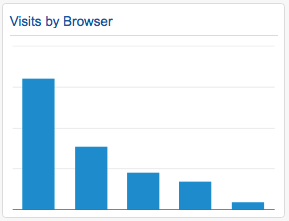
\includegraphics[scale=0.8]{img/bar-ver.png}
\caption{Pionowy układ słupków}\label{rys:wykres:pion}
\end{figure}

\begin{figure}[H]
\centering
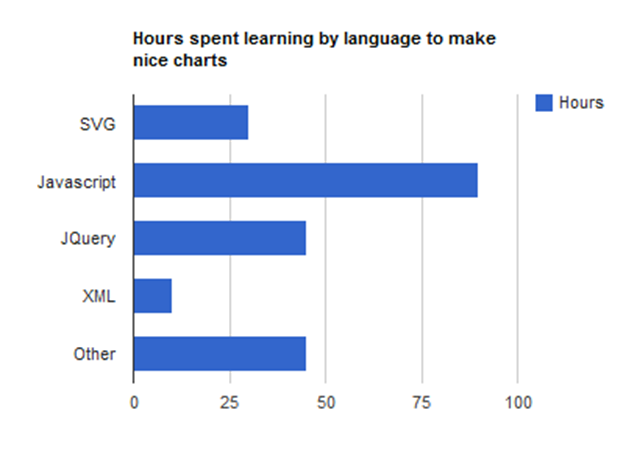
\includegraphics[scale=0.8]{img/bar-hor.png}
\caption{Poziomy układ słupków}\label{rys:wykres:poziom}
\end{figure}

\subsection{Stos}
Wykres słupkowy może zostać przedstawiony w~trybie stosowym. Wtedy dla każdej wartości z~dziedziny tworzony jest jeden słupek o~wysokości proporcjonalnej do sumy wartości próbek ze wszystkich serii wykresu. Z~kolei ten słupek jest podzielony na mniejsze cześci o~długościach i~kolorach odpowiednich próbek. Na rysunku~\ref{rys:wykres:stos} przedstawiam przykład stosowego wykresu słupkowego.

\begin{figure}[H]
\centering
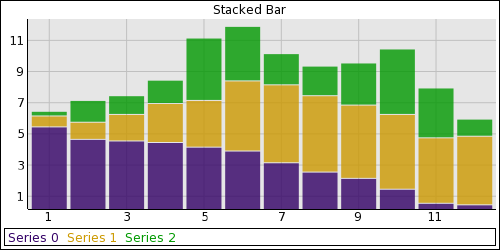
\includegraphics[scale=0.8]{img/stacked-bar.png}
\caption{Stosowy wykres słupkowy}\label{rys:wykres:stos}
\end{figure}


\section{Wykres liniowy}
W wykresie liniowym dana próbka jest prezentowana za pomocą pojedynczego punktu. Punkty są prezentowane jako koła o~zadanym promieniu. Wartości próbek należą do zbioru liczb rzeczywistych. Punkty danej serii mogą zostać połączone w~łamaną.

\subsection{Łączenie punktów}
Programista powinien mieć możliwość podjęcia wyboru w~kwestii łączenia punktów w~łamaną. Powinien mieć również możliwość zmiany wszystkich parametrów łamanej, tak jak dla elementów odpowiedzialnych za prezentację próbek.

\section{Dodatki}
Wszystkie opisane tu funkcjonalności są opcjonalne, a~ich realizacja nie jest konieczna do zakończenia prac nad biblioteką.

\subsection{Motywy}
Dodatkiem, który podniósłby atrakcyjność wykresów jest wysokopoziomowy mechanizm motywów, podobny do \textit{QStyle}. Mechanizm ten powinien umożliwiać tworzenie wykresów o~spójnej kolorystyce oraz czcionkach. Zmiana motywu dla danego wykresu powinna sprowadzać się do prostej operacji.

\subsection{Budowanie wykresu}
Powinno być możliwe animowanie procesu budowania wykresu. Podczas tego procesu kolejne elementy wykresu będą stawały się widoczne, a~elementy odpowiedzialne za prezentację danych powinny stopniowo przyjmować swoje wartości, począwszy od zera.

\subsection{Generowanie plików graficznych}
Powinno być możliwe generowanie na podstawie istniejących wykresów plików graficznych  w~formatach PNG i~SVG.

\section{Przenośność}
Biblioteka musi wpisywać się w~politykę Qt brzmiącą: \textit{pisz raz, kompiluj wielokrotnie}. Musi być przenośna na poziomie kodu źródłowego między najważniejszymi wspieranymi przez Qt platformami.
Minimum to uruchomienie na systemach:
\begin{itemize}
\item{Windows,}
\item{Linux.}
\end{itemize}


\section{Wymagania pozafunkcjonalne}
Wymagania funkcjonalne nie są jedynymi kryteriami oceny biblioteki. Równie ważne są wymagania definiujące oczekiwania użytkownika na temat budowy biblioteki oraz wynikające z~niej ograniczenia dotyczące wydajności czy skalowalności. Poniżej poruszam te i~kilka innych kwestii nie związanych bezpośrednio z~funkcjonalnością.

\subsection{API w stylu Qt}
%API tworzonej przeze mnie bilioteki powinno posiadać jak najwięcej z sześciu cech charakteryzujących %dobre interfejsy programistyczne:
%\begin{itemize}
%\item{minimalne,}
%\item{kompletne,}
%\item{intuicyjne,} 
%\item{łatwe do zapamiętania,}
%\item{czysta i~prosta semantyka,}
%\item{czytelny kod.}
%\end{itemize}

%Jednak nie są to wszystkie wymagania stawiane projektowanej bibliotece. 

Aby tworzony przeze mnie kod był czytelny dla innych programistów Qt, musi on wykorzystywać standardowe mechanizmy tej platformy:
\begin{itemize}
\item{statyczny polimorfizm, polegający na tworzeniu podobnych interfejsów dla podobnych, ale niespokrewnionych klas, np. kontenerów. Zastępuje wprowadzanie sztucznych klas bazowych.}
\item{właściwości jako sposób na parametryzowanie obiektów,}
\item{preferowanie przyjmowania wskaźników zamiast referencji do funkcji modyfikujących argumenty,}
\item{asynchroniczna komunikacja między obiektami rozwiązana za pomocą sygnałów i~slotów,}
\item{nazewnictwo, sposób zwracania wartości z~funkcji i~wiele innych opisanych w~\cite{APIDesign}.}
\end{itemize}

\subsection{Wymienność biblioteki}
Biblioteka powinna wykorzystywać mechanizmy pozwalające na tworzenie bibliotek dynamicznych wymiennych pomiędzy wersjami. Wprowadzenie nowej wersji biblioteki z~niezmienionym interfejsem nie powinno wymagać przebudowania całej aplikacji z~niej korzystającej.

\subsection{Nowoczesność i~uniwersalność}
Biblioteka powinna wykorzystywać możliwie nowe technologie, np. Qt5. Biblioteka może korzystać ze standardu \textit{C++11}, jednak nie powinna wymuszać na użytkowniku posiadania kompilatora zgodnego z~tym standardem. Komponenty dostarczane do użytku programistom powinny być możliwie wysokopoziomowe i~uniwersalne w~użyciu.

\subsection{Wydajność}
Jako, że okoliczności wykorzystania wykresów biurowych są inne niż wykresów technicznych oraz natura ich danych jest dużo bardziej statyczna, optymalizacja nie jest tu kwestią najważniejszą. 
Z~tego powodu, oraz z~chęci uniknięcia antywzorca projektowego przedwczesnej optymalizacji, kwestia wydajności bilioteki jest odsuwana na dalszy plan.

\subsection{Niezawodność}
Jak już wspomniałem w~poprzednim punkcie, natura oraz zastosowania wykresów biurowych różnią się od technicznych, a~co za tym idzie, mają również inne wymagania dotyczące niezawodności. Przewiduje się, że biblioteka będzie przeznaczona do aplikacji finansowych i~biurowych, a nie systemów czasu rzeczywistego. Tym niemniej, w~celu minimalizacji liczby błędów w~kodzie, powinny zostać zastosowane testy regresji. Zachowanie biblioteki w warunkach ekstremalnych, np. ograniczonego dostępu do zasobów, nie jest głównym celem projektu.

%\subsubsection{Wiarygodnosć}

\subsection{Skalowalność}
Zarówno dodawanie nowych jak i~usuwanie już istniejących elementów biblioteki powinno być łatwe i~nie powinno mieć wpływu na stabilność pracy biblioteki. Dodawanie nowych elementów powinno być możliwe dzięki uniwersalnym interfejsom. Natomiast usuwanie istniejących elementów powinno sprowadzać się do wyłączenia ich z~procesu budowania biblioteki.
